\chapter{Hardware}\label{ch:hardware}
- chapter will talk about challenges we faced in finding stable connectors\\
- material used: PLA (biodegradable, sturdy enough, ...)\\
- assembled based on ID system\\
- no special requirements to printer\\
- we used: UltiMaker3, UltiMaker2 and \info{remember name of other printer}

\section{Building Parts}
We can differentiate between three essential building parts for our truss structures. \textit{Links} are the connecting and shaping parts. We used PET bottles for these parts, because they are readily available, cheap and sturdy.\\
We have two different ways of connecting links. For dynamic connections, i.e. connections that allow movement of the structure, we use a hinge chain system. Rigid connections use single-part objects, we call \textit{hubs}.\\
Links, and hubs or hinge chains are connected by purpose-designed \textit{cuffs}, which fit over the bottles' thread and a connector part on the hub.

\subsection{Links}
We opted to use 1l (big) and 0.5l (small) reusable PET bottles because of their intrinsic stability and abundant availability. Two bottles are connected on their bottom side by a wood screw, which is inserted using a special long-necked screwdriver. The resulting link-lengths are:
\begin{enumerate}
\item 60 cm - two big bottles
\item 53 cm - one big and one small bottle
\item 46 cm - two small bottles
\end{enumerate}

\subsection{Hubs}

\subsection{Hinge Chains}
We are using truss structures specifically because of their structural stability. In order to introduce movement to these constructions, we came across some challenges. Multiple edges have to be able to pivot around a common hub. This kind of spherical can potentially achieved using ball joints. However, these typically only allow for a connection of two edges without obstructing each other.\\
We solve this issue by using a \textit{spherical joint mechanism}. As can be seen in Figure \ref{fig:hinge_chain}, these chains of hinges can connect multiple edges, which can all rotate around the same center. This is possible, because the axes of rotation do not occupy the rotational center itself, creating room for movement.\\
\begin{figure}[h!]
    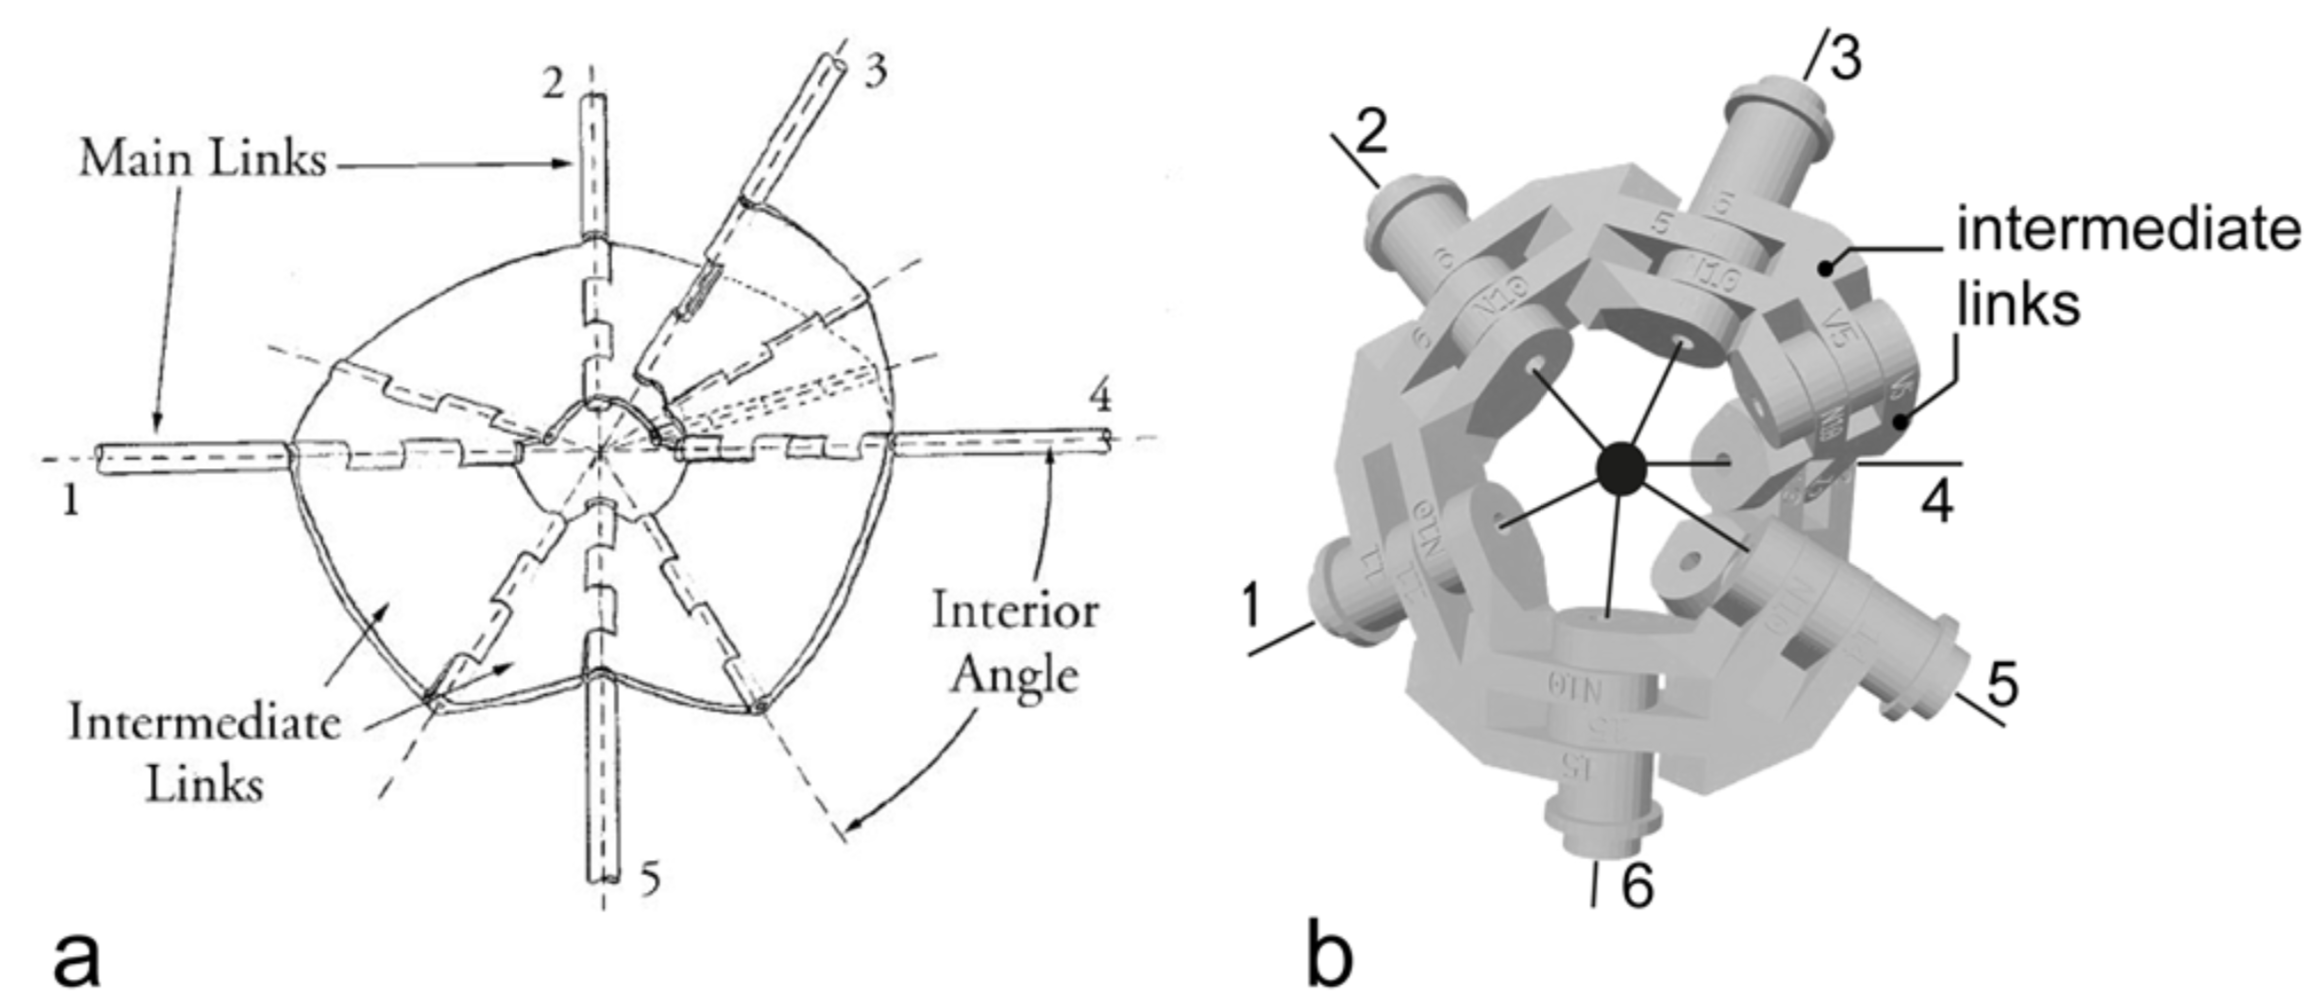
\includegraphics[width=\textwidth]{Hardware/hinge_chain.png}
    \centering
    \caption{(a) spherical joint mechanism connecting 5 edges. (b) rendering of TrussFabs' hinge chain design connecting 6 edges.}
    \label{fig:hinge_chain}
\end{figure}
We started out using an open hinge chain, meaning that the chain had special end parts which were not connected. This gave us a lot of freedom of movement, however it turned out that this design was not strong enough for our needs and frequently broke during testing builds of the T-Rex. This required us to rethink our design and we came up with a closed hinge chain.\\
The degrees of freedom (DoF), our hinge system needs to have, underly constraints, allowing us to limit the possible movement of the hinges. The original spherical joint mechanism shown in Figure \ref{fig:hinge_chain}a connected all edges using two hinges, allowing for 2 DoF. This is not necessary if we are dealing with truss structures. An example of TrussFabs's hinge design can be seen in Figure \ref{fig:hinge_chain}b. Only edge 4 is connected to its neighboring edges using two intermediate hinges. All other edges only require rotation (resulting in 1 DoF).\\


\subsection{Cuffs}
In order to connect links to nodes, we developed a custom coupling system. These cuffs fit exactly over the neck of the bottle and special connecting parts on the hubs.
- something about sizes of bottle neck\\
- size of connecting part\\
- little dimple for extra stability\\

\subsection{Stability}
The hinge parts and connecting cuffs are printed using consumer-grade desktop FDM\footnote{Fused Deposition Modeling} 3D printers. The filament consisted of PLA\footnote{Polylactic acid} plastic and the parts had a 15\% infill with a wall thickness of 3 mm. We chose PLA filament instead of ABS\footnote{Acrylonitrile butadiene styrene} primarily because of its easier usability. ABS plastic, while being stronger, needs to be printed on a heated surface, which many hobbyist printers do not have. As we designed our tool for 3D-printing enthusiasts and not professionals, we wanted to target owners of consumer-grade printers. Additionally, PLA consists of organic materials (mainly cornstarch and sugarcane), which makes it biodegradable, as opposed to ABS plastic, which is oil-based.\\
We aimed to make our software simulation as accurate to the real-world object as possible. To calibrate the simulation values, we therefore measured the forces of our T-Rex example.\\
\begin{figure}[h!]
    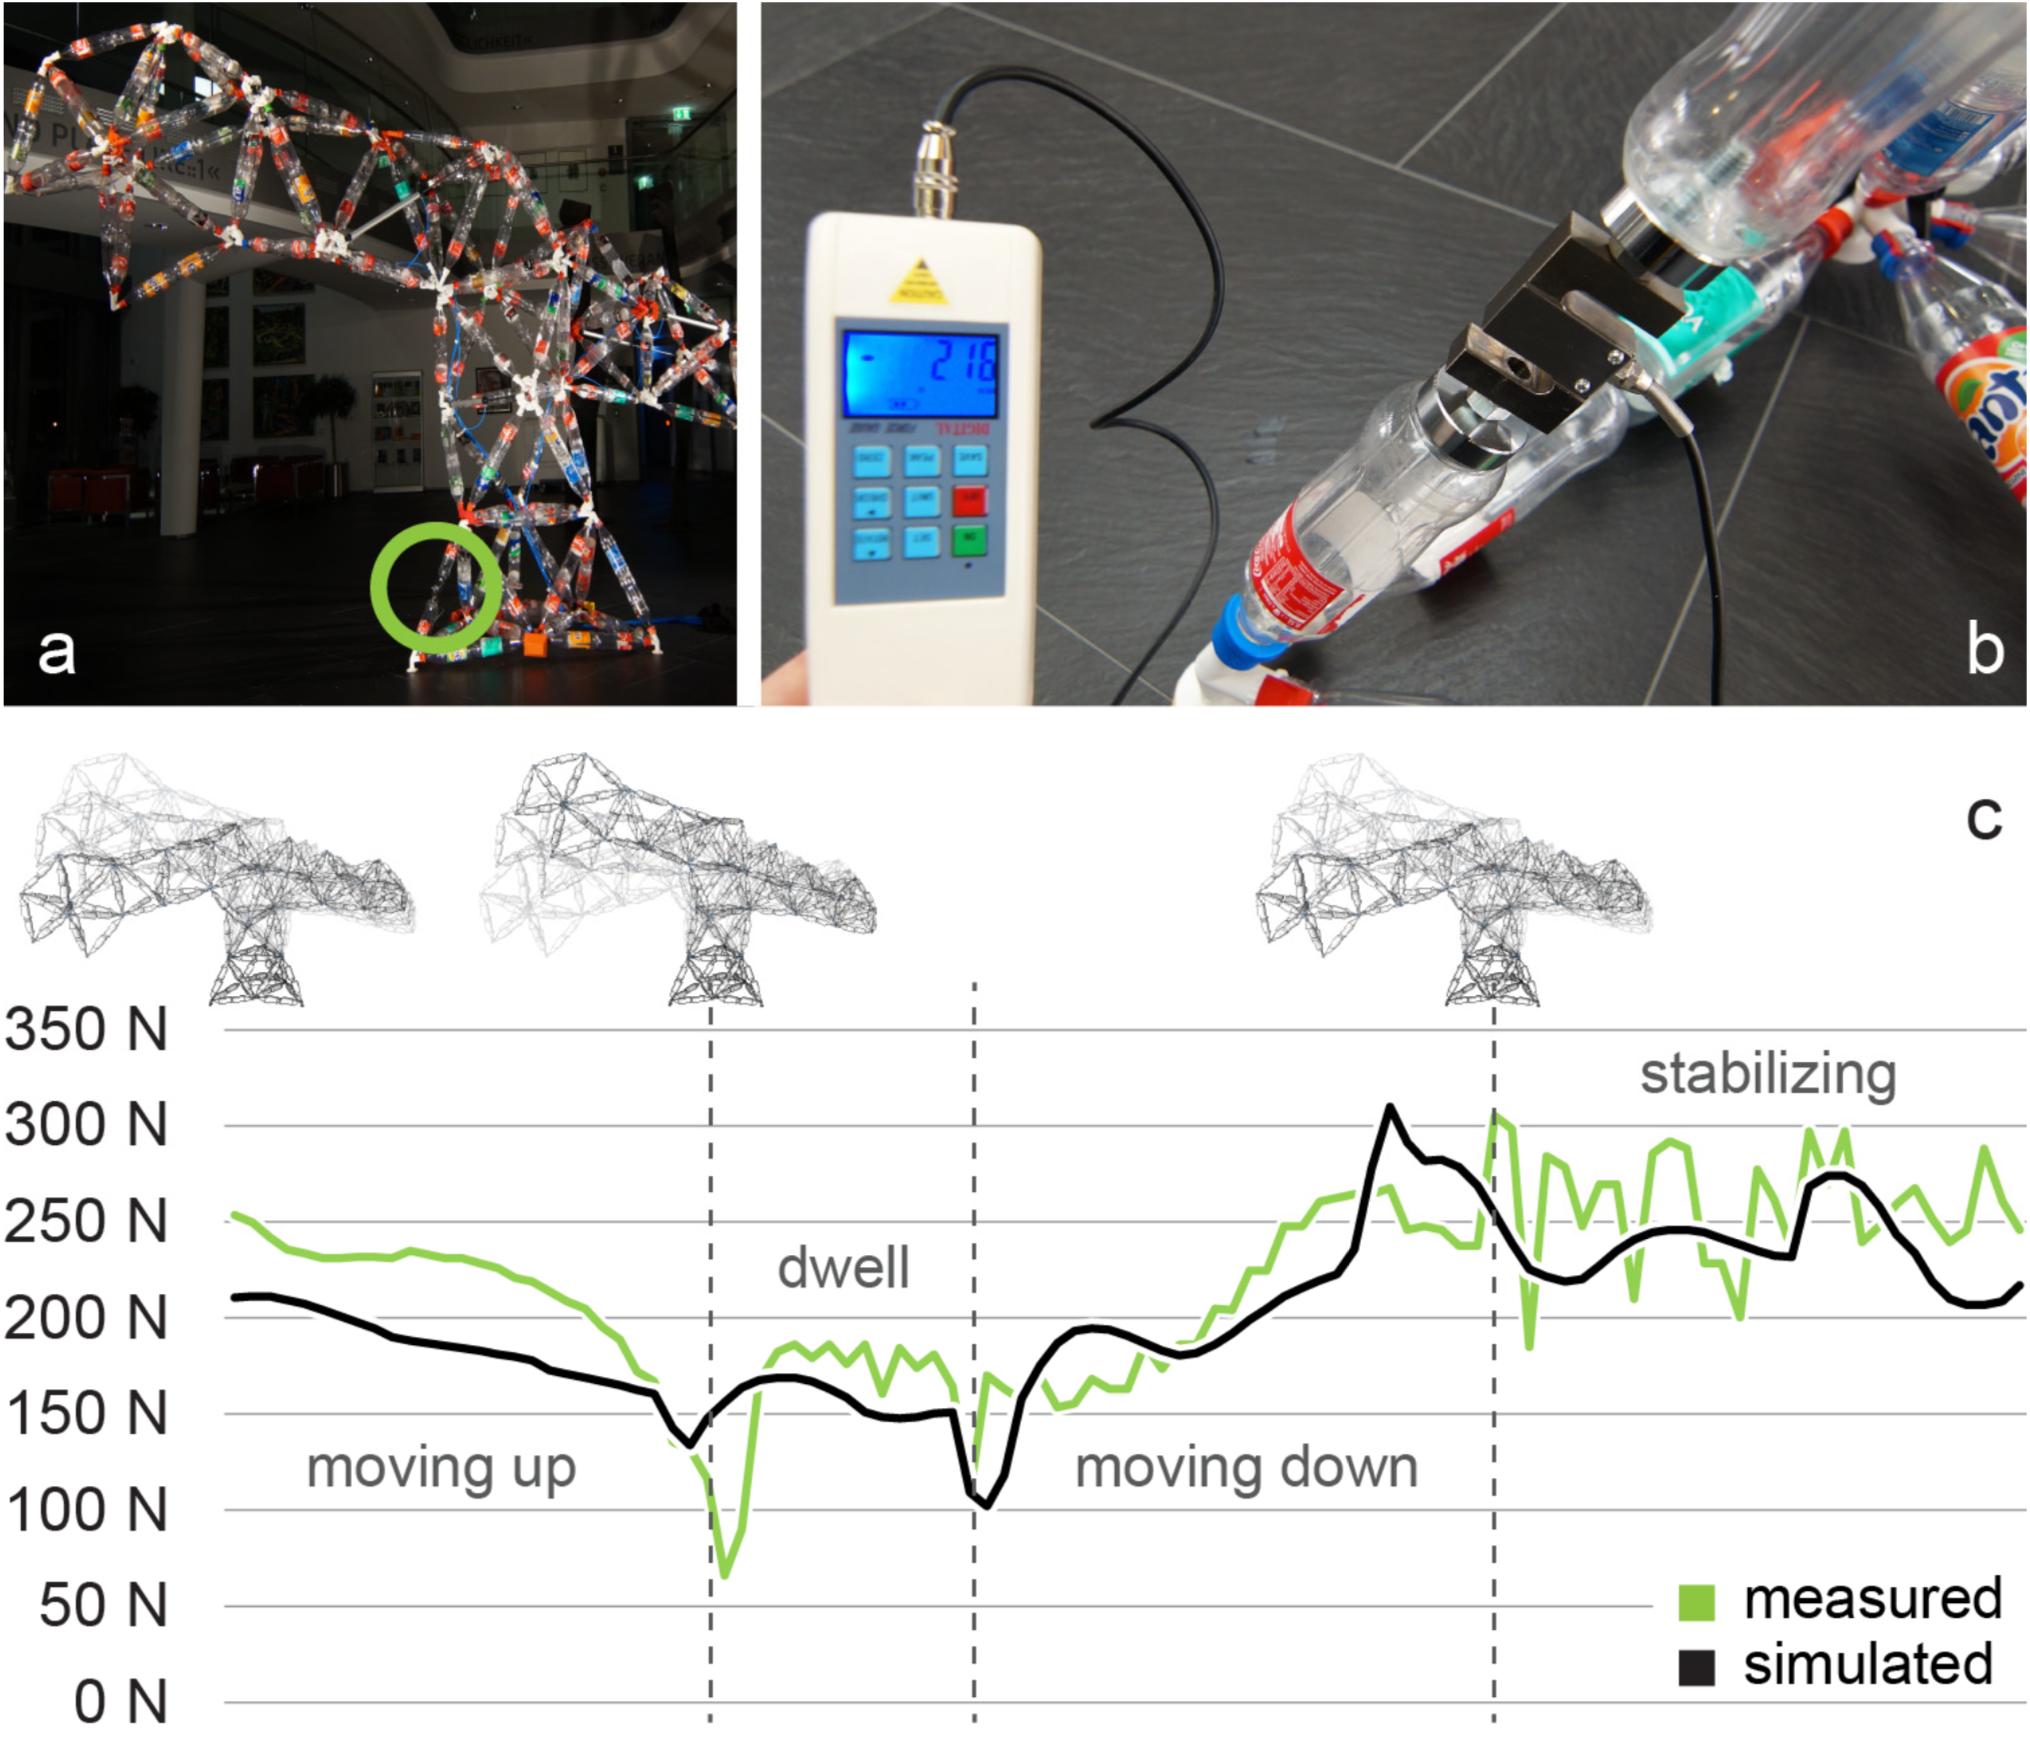
\includegraphics[width=\textwidth]{Hardware/force_measurement.png}
    \centering
    \caption{(a) We measured the forces on the bottom front edge of the T-Rex (b) using a digital force gauge. (c) The measured forces agree with the simulated forces.}
    \label{fig:force_measurement}
\end{figure}
We used a digital force sensor, with a capacity of 5000N and an error rate of 0.5\%, on the front bottom edge of the T-Rex (Figure \ref{fig:force_measurement} a-b). It was placed between two small bottles, giving the edge the same length as it would have had with two big bottles. We chose this position, because it bears the largest force due to the long lever force the neck of the T-Rex produces. Our test case consisted of moving the head up from its lowest to its highest and then back down to its lowest position again. The same movement, with the same speed, was programmed in the simulation. Figure \ref{fig:force_measurement}c shows, that both, the simulated and the measured force, are in agreement.

\section{Controls}
We controll the pneumatic actuators using a MIDI control interface. The slider inputs are sent to an Arduino which translats them to control signals for digitally controllable pressure valves. The actuators have two connections for air pipes: one for extending the actuator and one for retracting it. The signal from the slider is interpreted as a mixture between these two inputs, with the slider at the top meaning that all the air is send to the extending input and the slider at the bottom completely retracting it. This way we achieved manual open-loop position control.\\
\begin{figure}[h!]
    \includegraphics[width=\textwidth]{Hardware/hardware_setup.png}
    \centering
    \caption{Hardware setup for controlling the T-Rex, with Arduino, electric pressure control valves, and compressor.}
    \label{fig:hardware_setup}
\end{figure}
Figure \ref{fig:hardware_setup} shows the main parts of our hardware setup. The electrically controllable pressure regulators receive signals from the control board and limit the air pressure according to the needed level of extension of a given actuator. One pressure regulator is connected to exactly on actuator. The \textit{Airpress HL 360} compressor delivers the regulators with up to 8 bars of pressure.\\
The limited pressure is tunneled to a valve terminal. This terminal opens and closes airflow to the actuators. If it opens a valve, the regulated pressure will enter its air circuit and change the extension of the actuator. If it closes it, the pressure will stay constant and the actuator keeps its position.

\subsection{Electric vs. Pneumatic Actuators}
Early TrussFab prototypes used electric actuators, instead of the pneumatic ones we used for the T-Rex. Electric actuators can produce a fairly large force and are easier to control, as they can usually provide their current extension. However, at around 0.03 m/s they extend very slowly, compared to our pneumatic actuators, which can reach up to 20 m/s. As our structures are fairly lightweight, the force of the actuators is not a big concern, while the higher speed of pneumatic actuators enables us to create more dynamic structures.

\subsection{Open Loop vs. Closed Loop}
The MIDI controller is a well working possibility to control the actuators. It is, however, still a closed-loop control, meaning it can not react to external influences, like weight shifts or additional pressure acting on edges. This is not a big problem for our T-Rex example, as it usually moves mostly undisturbed and stand-alone. If we want to create an interactive object, this will not be sufficient.\todo{check if this is right}\\
Pneumatic actuators on their own tend to not have the possibility to measure their own rate of extension. We therefore created an easy to build distance sensor, using a string on a spindle. One side of the string is attached to the piston part of the actuator, while the spindle is attached to the static body. While the actuator extends, the spindle will spin, releasing more string. We attached a rotary encoder to the spindle, that can count the turns of the spindle. Using the diameter of the reel, we can calculate how much string was released during the extension, which correlates with the extension of the piston itself.\\
Using this approach, we can have closed-loop control of the actuators, making it possible to constantly monitor its the extension and applying force accordingly.\\
We created a rudimentary motion-platform using closed-loop PID control (s.a. Section \ref{sec:pid}). The motion platform had three modes. It started fully extended, applying a little bit of force to keep the actuator upright, but little enough that a human sitting on it pushed it back. If the actuator reached an extension of 10 cm, the control loop applied a holding force, making it possible to sit on the platform without it moving. If the human applied more force, pushing the piston further down, the third mode activated, making the motion platform oscillate up and down.
